%
% File naaclhlt2016.tex
%

\documentclass[11pt,letterpaper]{article}
\usepackage{naaclhlt2016}
\usepackage{times}
\usepackage{latexsym}
\usepackage{graphicx}
\usepackage{subcaption}
\usepackage{tabularx}

% \naaclfinalcopy % Uncomment this line for the final submission
\def\naaclpaperid{***} %  Enter the naacl Paper ID here

% To expand the titlebox for more authors, uncomment
% below and set accordingly.
% \addtolength\titlebox{.5in}    

\newcommand\BibTeX{B{\sc ib}\TeX}


\title{Crowdsourcing for (almost) Real-time Question Answering}

% Author information can be set in various styles:
% For several authors from the same institution:
% \author{Author 1 \and ... \and Author n \\
%         Address line \\ ... \\ Address line}
% if the names do not fit well on one line use
%         Author 1 \\ {\bf Author 2} \\ ... \\ {\bf Author n} \\
% For authors from different institutions:
% \author{Author 1 \\ Address line \\  ... \\ Address line
%         \And  ... \And
%         Author n \\ Address line \\ ... \\ Address line}
% To start a seperate ``row'' of authors use \AND, as in
% \author{Author 1 \\ Address line \\  ... \\ Address line
%         \AND
%         Author 2 \\ Address line \\ ... \\ Address line \And
%         Author 3 \\ Address line \\ ... \\ Address line}
% If the title and author information does not fit in the area allocated,
% place \setlength\titlebox{<new height>} right after
% at the top, where <new height> can be something larger than 2.25in

\author{Denis Savenkov \\ Emory University \\ {\tt dsavenk@emory.edu} 
  \And Scott Weitzner \\ Emory University \\ {\tt sweitzn@emory.edu}
  \And Eugene Agichtein \\ Emory University \\ {\tt eugene@mathcs.emory.edu}
}

\date{}

\begin{document}

\maketitle

\begin{abstract}

Modern search engines have made dramatic progress in answering many of user's questions about facts, such as those that might be retrieved or directly inferred from a knowledge base. However, many other questions that real users ask are more complex, such as asking for opinions or advice for a particular situation, and are still largely beyond the competence of the computer systems.
As conversational agents become more popular, QA systems are increasingly expected to handle such complex questions, and to do so in (nearly) real-time, as the searcher is unlikely to wait longer than a minute or two for an answer.
One way to overcome some of the challenges in complex question answering is crowdsourcing.
We explore two ways crowdsourcing can assist a question answering system that operates in (near) real time: by providing answer validation, which could be used to filter or re-rank the candidate answers, and by creating the answer candidates directly. Specifically, we focus on understanding the effects of time restrictions in the near real-time QA setting. Our experiments show that even within one minute time limit, crowd workers can produce reliable ratings for up to three answer candidates, and generate answers that slightly better than the (automated) winning system of the LiveQA 2015 shared task.
Our findings can be useful for developing hybdrid human-computer systems for automatic question answering and conversational agents.

\end{abstract}

\section{Introduction}
\label{sec:introduction}

It has long been a dream to communicate with a computer as with another human being using natural language speech and text.
Nowadays, we are coming closer to this dream, as natural language interfaces become increasingly popular.
Our phones are already reasonably good in recognizing speech, and personal assistants, such as Apple Siri, Google Now, Microsoft Cortana, Amazon Alexa, etc., help us with everyday tasks and answer some of our questions.
Chat bots are arguably considered ``the next big thing'', and a number startups developing this kind of technologies has emerged in Silicon Valley and around the world\footnote{http://time.com/4194063/chatbots-facebook-messenger-kik-wechat/}.

Question answering is one of the major components of such personal assistants.
Existing techniques already allow users to get direct answers to their factoid questions\footnote{https://www.stonetemple.com/rich-answers-in-search/}.
However, there is still a large number of more complex questions, such as advice or accepted general opinions, for which users have to dig into the ``10 blue links'' and extract or synthesize answers from information buried within the retrieved documents. To answer these information needs, community question answering (CQA) sites emerged, such as Yahoo! Answers and Stackexchange. These sites provide a popular way to connect information seekers with answerers. Unfortunately, it it can take minutes or hours, and sometimes days, for the community to respond, and some questions are left unanswered altogether. 

To address this challege, a recent TREC LiveQA 2015 shared task (www.trec-liveqa.org), where automated systems attempted to answer real users' questions within 1 minute. This task was successful, with the winning system able to automatically return a reasonable answer to more than half of the submitted questions. 



In this work we explore two ways common crowdsourcing can be used to help an automated system to answer complex user questions in near real-time scenario, e.g., within a minute.
More specifically, we study if crowd workers can authentically judge the quality of the proposed answer candidates, and if it is possible to obtain reasonable written answers from the crowd within a limited amount of time.

The research questions we study in this work are:
\begin{enumerate}
\item RQ1. Can crowdsourcing be used to judge the quality of answers to non-factoid questions under a time limit?
\item RQ2. Is it possible to use crowdsourcing to collect answers to real user questions under a time limit?
\item RQ3. How does the quality of crowdsourced answers to non-factoid question compare to original CQA answers, and to automatic answers from TREC LiveQA systems?
\end{enumerate}


\section{Methodology}
\label{sec:methodology}

To answer the research questions we conducted a series of crowdsourcing experiments using Amazon Mechanical Turk platform\footnote{http://mturk.com}.
We used questions from the TREC LiveQA 2015\footnote{http://trec-liveqa.org} shared task along with the system answers, rated by the NIST assessors\footnote{https://sites.google.com/site/trecliveqa2016/liveqa-qrels-2015}.
The questions for the task were selected by the organizers from the live stream of questions posted to Yahoo! Answers CQA platform on the day of the challenge (August 31, 2015).
For these questions we also crawled their answers, that were eventually posted on Yahoo! Answers\footnote{As the answer we took the top question, which may or may not have been selected as the ``Best answer'' by the author of the question.}.

To answer the RQ1 we asked workers to rate answers to a sample of 100 questions using official TREC rating scale:
\begin{enumerate}
\item 1: Bad - contains no useful information
\item 2: Fair - marginally useful information
\item 3: Good - partially answers the question
\item 4: Excellent - fully answers the question
\end{enumerate}

\begin{figure}[h!]
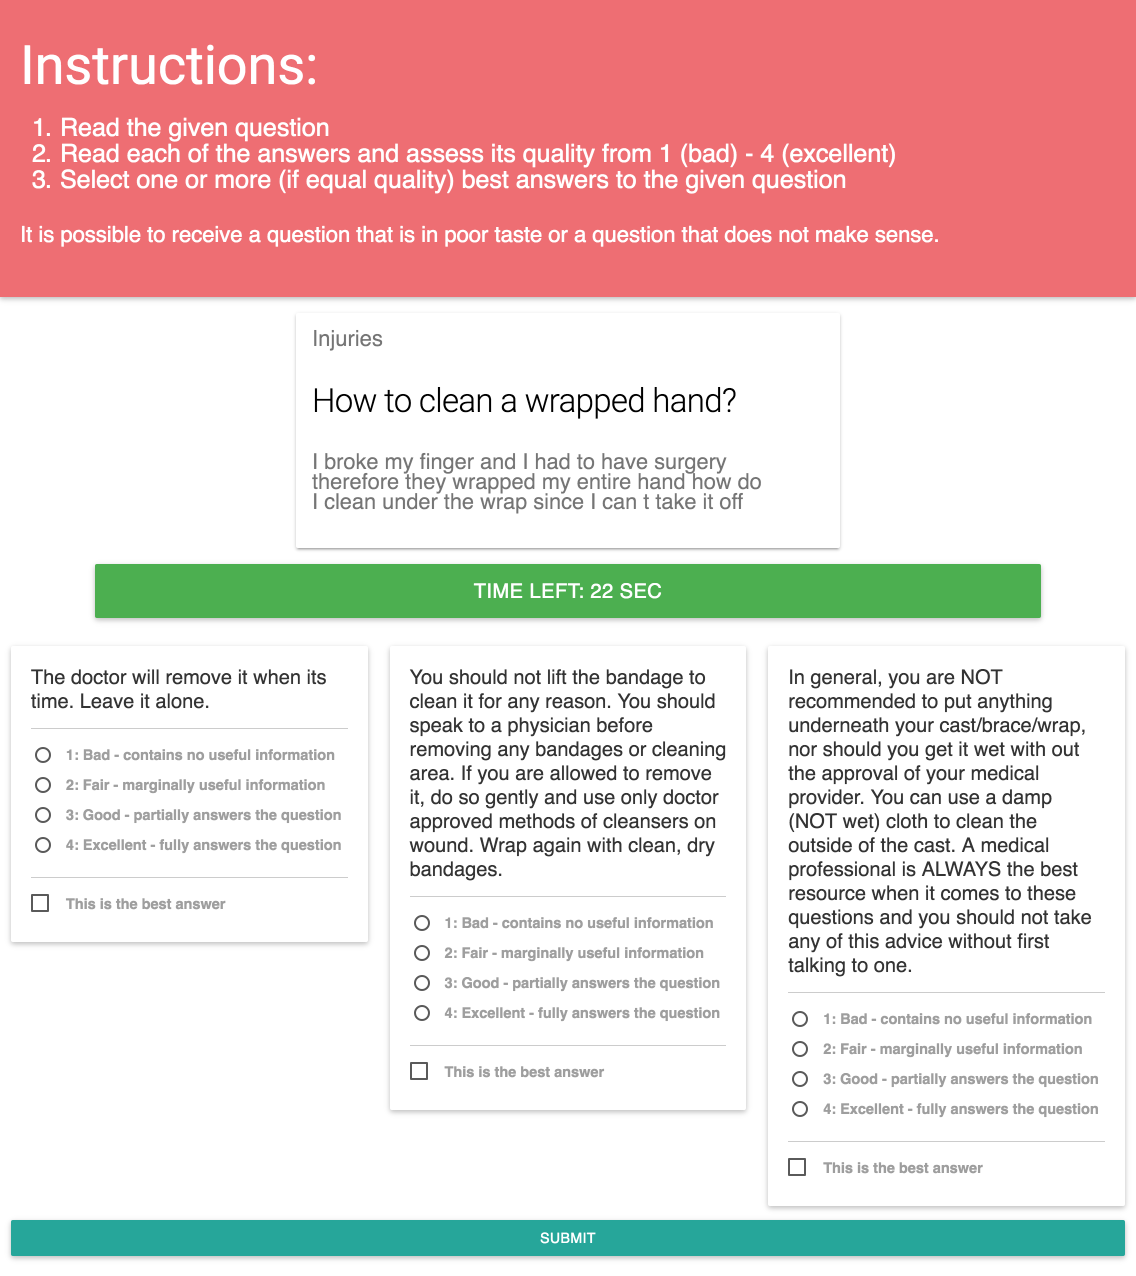
\includegraphics[width=1.0\linewidth]{img/validation_screenshot}
\caption{Answer validation form}
\label{fig:interfaces:validation}
\end{figure}

\begin{figure}[h!]
\centering
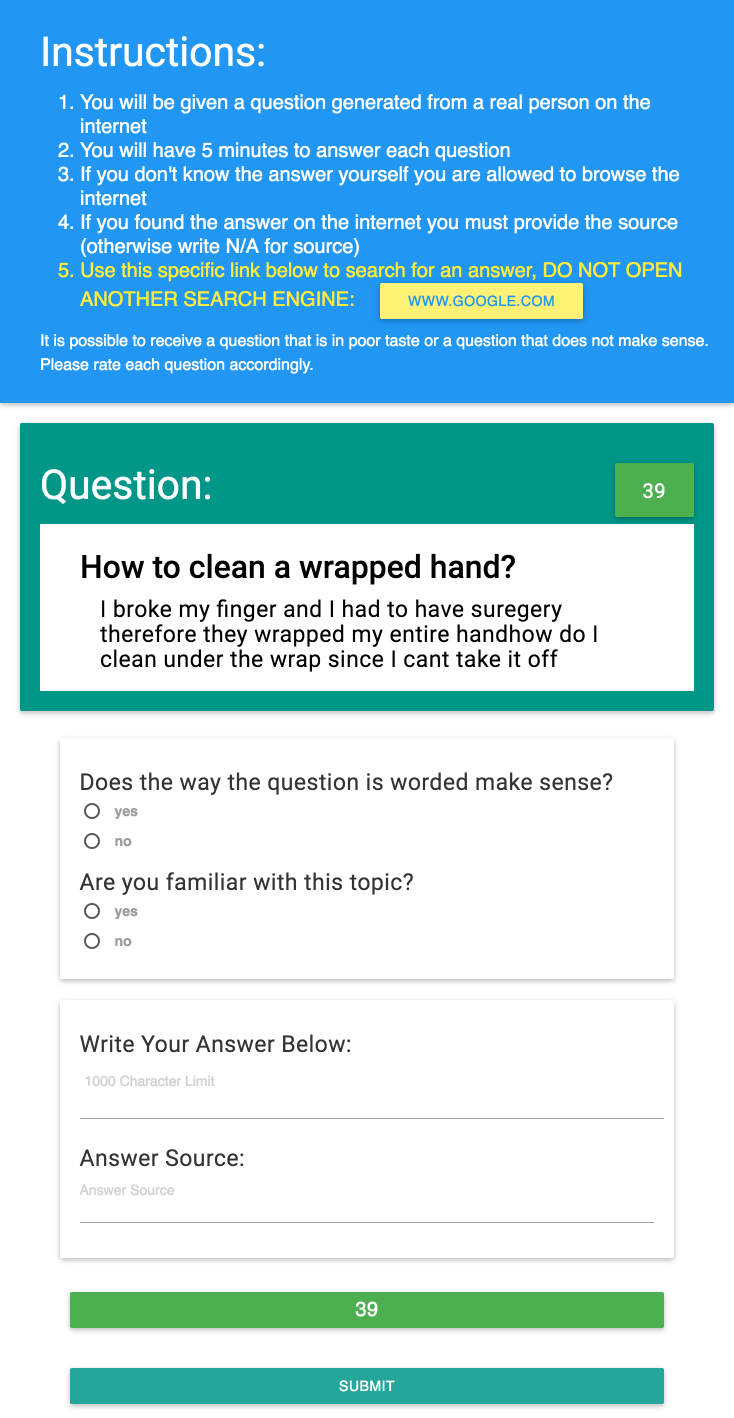
\includegraphics[width=0.9\linewidth]{img/answering_screenshot2}
\caption{Answer crowdsourcing form}
\label{fig:interfaces:answer}
\end{figure}


% \begin{figure*}[ht!]
% \centering

% \caption{Mechanical turk HTML forms for data collection}
% \label{fig:interfaces}
% \end{figure*}

We chose to display 3 answers for the question, which were generated by top-10 automatic systems from TREC LiveQA 2015 \cite{overviewliveqa15}.
To study the effect of time pressure on the quality of judgments we split participants into two groups, and one group made their assessments with a 1 minute countdown timer shown to them, while the other could do the task without worrying about time.
Within each group, we assigned three different workers per question.
The workers were compensated at a rate of \$0.05 per question for this task.

The interface for collecting answer ratings is shown on Figure \ref{fig:interfaces:validation}\footnote{The screenshots show the final state of the form, as we describe later in this sections fields were unhidden step by step for proper timing of reading, answering and validation}.
On top of the interface workers were shown the instructions on the task, and question and answers were hidden at this time.
They were instructed to read the question, read answers and rate their quality on a scale from 1 (Bad) to 4 (Excellent), and finally choose a subset of candidates that best answer the question.
Upon clicking a button to indicate that they were done reading the instructions, a question, a 60 second countdown timer, and 3 answers to the question appeared on the screen.
At the 15 second mark the timer color changed from the green to red.
In the experiments without time pressure the timer was hidden, but we still track the time it took the workers to complete the task.

To answer RQ2, we asked different workers to answer the questions from TREC LiveQA 2015.
Again, since we wanted to explore the abilities of crowdsourcing the answers in a real-time scenario, we split the workers into two groups and enforced a 1 minute time limit for one of them.
The form for answer crowdsourcing is shown on Figure \ref{fig:interfaces:answer}, and similar to the answer rating form it starts with a set of instructions on the task.
We let the users browse the internet if they aren't familiar with the topic and couldn't answer the question themselves.
To prevent them from finding the original question from Yahoo! Answers we included a link to Google search engine with date filter turned on\footnote{https://www.google.com/webhp?tbs=cdr:1,cd\_max:8/30/2015}.
Using this link workers could search the web as it was on 8/30/2015, before TREC LiveQA 2015 questions were posted and therefore workers were in the same conditions as automatic systems on the day of challenge\footnote{The ranking of search results could be different on the day of the challenge and for our workers}.
Initially, the question was hidden for proper accounting of question reading and answering times.
Upon clicking a button to indicate that they were done reading the instructions, a question appeared along with a button, which needs to be clicked when they done reading the question.
After that, the answering form appears, it contained four fields:
\begin{enumerate}
\item Does the answer make sense: A yes or no question to see if the answer was comprehensible 
\item Are you familiar with the question: A yes or no question to evaluate whether the worker has had prior knowledge regarding the question
\item Answer: the field to be used for the user's answer to the given question
\item Source: the source used to find the answer: URL of a webpage or NA if the worker used his own expertise
\end{enumerate}

For time-pressured collection users were shown a timer that counted down from 60 seconds after indicating they were done reading the question.
The timer changed from the color green to red once the timer reached 10 seconds.
The workers received a \$0.10 compensation for each answer.

Finally, to answer RQ3 we collected together crowdsourced answers, answers from the winning and another top-10 LiveQA'15 systems and the original answers crawled from Yahoo! Answers.
Each set of answers was given to mechanical turk workers for rating, and we collected 3 scores for each of them.


\section{Results and Discussion}
\label{sec:results}

In this section we will describe our results and discuss some of the implications.
We start from results on answer rating (Section \ref{subsec:results:answer_rating}), and then describe the answer crowdsourcing experiment (Section \ref{subsec:results:answer_crowd}).

\subsection{Answer rating}
\label{subsec:results:answer_rating}

In the answer rating experiment we collected 6 ratings (3 with and without time pressure) for each of three answers for a sample of 100 questions, which makes it a total of 900 judgments.
Each of the answers also has an official NIST assessor rating on the same scale.
Figure \ref{figure:score_correlation} shows correlation between official NIST assessor relevance judgments and ratings provided by our workers.
The Pearson correlation between the scores is $\rho=0.52$.
The distribution of scores shows, that official assessors were very strict and assigned many extreme scores of 1 or 4, whereas mechanical turk workers preferred intermediate scores of 2 and 3.
The results did not show any significant differences between experiments with and without time pressure.
Therefore, for RQ1 we conclude that on average one minute is enough to judge three answers to CQA questions.


\begin{figure}[t!]
	\centering
	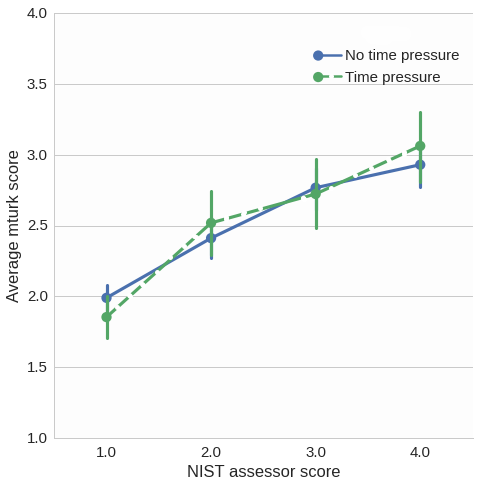
\includegraphics[width=0.4\textwidth]{img/score_correlation}
	\caption{Correlation between NIST assessor scores and crowdsourced ratings with and without time limit on the work time}
	\label{figure:score_correlation}
\end{figure}
	

Figure \ref{figure:validation_time} shows that even though the median time to rate all three answers is around 22-25 seconds in both experiments, the upper bound is significantly lower in the experiment with the time pressure.

\begin{figure}[t!]
	\centering
	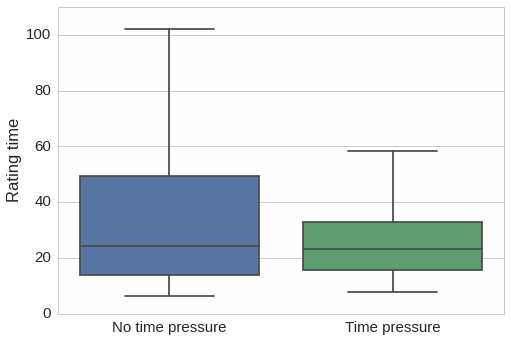
\includegraphics[width=0.5\textwidth]{img/validation_time}
	\caption{Box plot of answer rating time with and without time pressure}
	\label{figure:validation_time}
\end{figure}

We can conclude, that in general we can trust crowdsourced ratings and we will use them in our next experiment to estimate the quality of different answers.

\subsection{Answer crowdsourcing}
\label{subsec:results:answer_crowd}

In our experiment in answer crowdsourcing we collected 6 answers (with and without time pressure) for each of the 1087 LiveQA'15 questions.
Since we have answers from different sources, let's make the following notations:
\begin{itemize}
	\item \textit{Yahoo! Answers} - answers eventually posted by users on Yahoo! Answers for the original questions
	\item \textit{Crowd} - answers collected from Mechanical Turk workers without time pressure
	\item \textit{Crowd-time} - answers collected from Mechanical Turk workers with one minute time pressure
	\item \textit{LiveQA winner} - answers from the TREC LiveQA'15 winning system
	\item \textit{LiveQA top10} - answers from another top 10 TREC LiveQA'15 system.
\end{itemize}

%\footnote{We will release the data for the community???}.
Table \ref{table:answer_stats} summarizes some statistics on the answers.
First thing to notice is that, unlike CQA websites, where some questions are left unanswered, by paying the crowd workers we were able to get at least one answer for all LiveQA questions (after filtering ``NA'' and ``I don't know'' answers).
The length of the answers, provided by Mechanical turk users is lower, and time pressure forces user to be even more concise.
The majority of workers ($\sim90 \%$) didn't use the web search and provided answers based on their experience and common knowledge.

\begin{table*}[h!t]
\centering
\caption{Statistics of different types of answers for Yahoo! Answers questions}
\begin{tabular}{| p{3cm} | c | c | c | c |}
\hline
Statistic & Y!A & mTurk & mTurk-time & LiveQA'15 winning system\\
\hline
\% answered & 78.7\% & 100.0\% & 100.0\% & 97.8\% \\
Length (chars) & 354.96 & 190.83 & 126.65 & 790.41 \\
Length (words) & 64.54 & 34.16 & 22.82 & 137.23 \\
\hline
\end{tabular}
\label{table:answer_stats}
\end{table*}

From the Figure \ref{fig:answering_time_distribution} we can see that adding time pressure shifts the distribution of answering times\footnote{For the experiment with time pressure we had separate timers for reading instructions, reading the question and writing the answer, that's why the total time on the plot could be more than 1 minute}.

\begin{figure}[h]
	\centering
	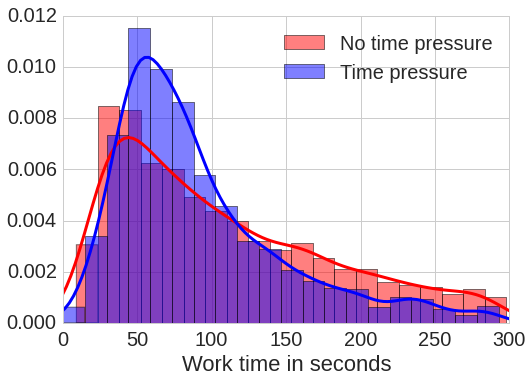
\includegraphics[width=0.5\textwidth]{img/answering_time_distribution}
	\caption{Distribution of answering times for experiments with and without time pressure}
	\label{fig:answering_time_distribution}
\end{figure}

To answer RQ2 and RQ3 and estimate the quality of answers, we took a sample of 100 questions and repeated the answer rating experiment on this data.
Each answer was judged by 3 different workers, and their scores were averaged.
Figure \ref{fig:average_score} displays the plot with average score for answers from different sources.
Quite surprisingly the quality of collected answers turned out be comparable to answers provided by the CQA website users.
Average rating of answers produced by the winning TREC LiveQA system is also pretty close to those of human answers.
Finally, as expected, time pressure had its negative effect on the quality.

\begin{figure}[h]
	\centering
	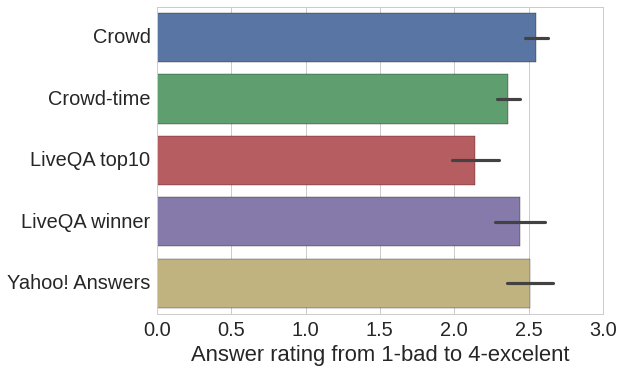
\includegraphics[width=0.5\textwidth]{img/average_score}
	\caption{Average scores of different type of answers to Yahoo! Answers questions for different categories}
	\label{fig:average_score}
\end{figure}

Analysis of scores distribution (Figure \ref{fig:scores_distribution}) shed some light on the nature of the problems with automatic and human answers.
As we can see, automatic systems generate non-relevant answers ($score=1$) more often than human.
This means, that quite often the model either fails to retrieve relevant information or to separate between useful and non-useful answer candidates.
However, by having larger information store, e.g. world wide web, question answering systems can often find the perfect answer ($score=4$), while regular people tend to give generally useful responses ($score=2,3$).
Table \ref{table:answer_examples} gives some example answers from different sources.

\begin{figure}[h]
\centering
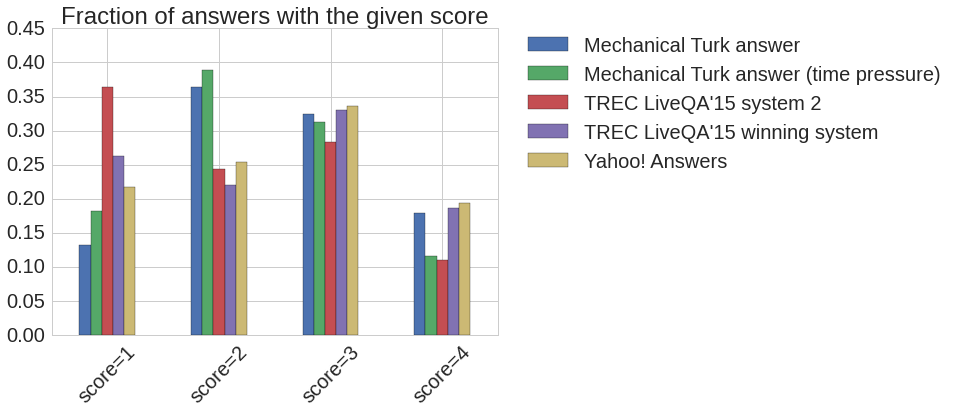
\includegraphics[width=0.5\textwidth]{img/scores_distribution}
\caption{Distribution of scores for different types of answers to Yahoo! Answers questions}
\label{fig:scores_distribution}
\end{figure}


\begin{table*}[h!t]
\centering
\caption{Examples of answers to some of the TREC LiveQA'15 questions}
\begin{tabular}{| p{3cm} | p{12.5cm} |}
\hline
 & Answer \\
\hline
\hline
\multicolumn{2}{|c|}{How long do Rottweilers usually live?} \\
\hline
Yahoo! Answer & I'm afraid anything from about 7 to 12.... some we lose outside of those ages such as 5 or 15 but they are extreme.\\
Crowd & The average life expectancy of a rottweiler is about 9 years. Smaller breeds have higher life expectancies\\
Crowd-time & Any where between 8-12 years\\
LiveQA winner & Here's an answer to your question and some other information you may find useful. Average Life Span: 10-13 years Average Weight: Male 110 pounds, Females 90 pounds Color And Coat: Coarse flat coat, black in color with rust markings on cheeks, muzzle, chest, legs, above eyes and under the tail. Typical Health Problems: ...\\
\hline
\hline
\multicolumn{2}{|c|}{Can Hammerli ar20 air rifle be used in a competition?}\\
\hline
Yahoo! Answers & You're not going to see them in international(Olympic, WC) 10M competition, but the Hammerli AR20 is a good starter rifle for young folks looking to get into the sport. Adult / starter 10M rifle If you're looking to get into the sport on the cheap. I suggest a S/H Feinwerkbau 300*** The FWB 300 is just as accurate as a new 700 or 800. The 300 just has fewer bells and whistles. At 1/5th the cost(or less) though, you can't beat the price for performance. ***have someone that knows what to look for examine the rifle for you.\\
Crowd & Yes they can be. Not everything can be in all competitions but this gun can certainly be in some.\\
Crowd-time & Yes\\
LiveQA winner & Ambidextrous cocking piece with release lever. Wide loading recess with precision feed. Lothar Walther match barrel. Silver aluminum stock with variable stock length, cheekpiece height and fore end height. Ambidextrous grip and stock. Shorten or lengthen the stock with included spacers (41.65" to 43.66"). Front sight globe accepts 3.8mm inserts (1 insert included). Fully adjustable diopter rear sight. 29.53" (750mm) sight length, 200 and 300 bar fill pressures (2,900 psi and 4,351 psi, respectively). Removable aluminum air cylinder with integral manometer (air pressure gauge). 2-stage trigger can be adjusted for pressure point, pull weight, stop and slack. T-rail for 3-position competition\\
\hline
\end{tabular}
\label{table:answer_examples}
\end{table*}


Our analysis suggests that regular people can quickly give a reasonable answer to CQA questions.
Of course, in many case an certain expertise is required to answer a question, which a random crowd worker might not possess.
However, in such cases it is possible to design a QA support system, which a worker can use in order to find the answer.
For example, in our experiment we let workers use web search to find answers, if they were unfamiliar with the topic, and more efficient interfaces are definitely possible.
We should note, that in many cases answer rating requires domain expertise as well, but we didn't focus on this aspect in the current work.
An answer might look reasonably relevant, but totally wrong.

An interesting question, that we leave for future work is how an automatic question answering system can put a human in the loop to improve the performance, and how it can utilize different kinds of data a user can quickly produce to be able to generate a reasonable answer while maintaining a near real-time response.
An automated system, that includes crowdsourcing in the loop needs to deal with the above mentioned trustworthiness issues.
A user, who receives an answer from an expert system will probably trust it more, than if the answer is provided by a random stranger on the internet.


\section{Related Work}
\label{sec:related_work}

Using the wisdom of a crowd to help users satisfy their information needs has been studied before in the literature.
\cite{bernstein2012direct} explored the use of crowdsourcing for offline preparation of answers to tail search queries.
In this work log mining techniques were used to identify potential question-answer fragment pairs, which were then processed by the crowd to generate the final answer.
This offline procedure allows a search engine to increase the coverage of direct answers in response to user questions.
In our work, however, the focus is on online question answering, which requires fast responses to the user, who is unlikely to wait more than a minute.
Another related work is targeting a different domain of SQL queries.
The CrowdDB system \cite{franklin2011crowddb} is an SQL-like processing system for queries, that cannot be answered by machines only.
In CrowdDB human input is used to collect missing data, perform computationally difficult functions or matching against the query.
In \cite{aydin2014crowdsourcing} authors explored efficient ways to combine human input for multiple choice questions from the ``Who wants to be a millionaire?'' TV show.
In this scenario going with the majority for complex questions isn't effective, and certain answerer confidence weighting schemas can improve the results.  

Using crowdsourcing for relevance judgments has been studied extensively in the information retrieval community, e.g. \cite{Alonso:2008:CRE:1480506.1480508,alonso2011design,grady2010crowdsourcing}.


Crowdsourcing is usually associated with offline data collection, which requires certain amount of time for data collection.
Using crowdsourcing in (near) real-time scenarios poses certain additional challenges.
\cite{bernstein2011crowds} introduced the retainer model for recruiting synchronous crowds for interactive real-time tasks and showed their effectiveness on the best single image and creative generation tasks.
We are planning to build on this ideas to integrate a crowd into a real-time question answering system.
The work of \cite{Lasecki:2013:CCC:2501988.2502057} showed how multiple workers can sit behind a conversational agent named Chorus, where human input is used to propose and vote on responses. 


\section{Conclusion}
\label{sec:conclusion}

In this work we conducted a series of crowdsourcing experiments, designed to explore the potential usefulness of crowdsourcing for near real-time question answering.
The data we collected demonstrated, that crowd workers are capable of validating a small set of answer candidates within one minute time limit.
This can be used by an automatic QA system for answer validation and reranking.
In addition, one minute seems to be enough for a crowd to generate a fair or good response to the question (RQ2), which can be useful in case a QA system didn't have good candidates in the first place.
Finally, we compared crowdsourced answers with original Yahoo! Answers response and responses of LiveQA'15 systems (RQ3).
The quality of such answers on average turned out to be comparable to the original Yahoo! Answers responses, and even with time pressure crowdsourcing could potentially be useful for automatic systems.

%\section*{Acknowledgments}
%If any...

\bibliography{naaclhlt2016}
\bibliographystyle{naaclhlt2016}


\end{document}
